\subsection{Risikomanagement}
\textit{(pro)} In diesem Kapitel wird die Vorgehensweise des verwendeten Risikomanagement Modells erklärt. Die Durchführung eines Risikomanagements dient nebst der einfacheren Bewältigung von eintretenden Risikosituationen, der Sensibilisierung aller am Projekt beteiligten Personen auf allfällige Gefahrenquellen rund um die Projektarbeit. Das Risikomanagement besteht dabei aus mehreren Prozessen welche beachtet werden müssen. In Abb. \ref{fig:Risikomanagement} ist der Prozessaublauf illustriert welcher in diesem Projekt eingehalten wurde.

\begin{figure}[H]
	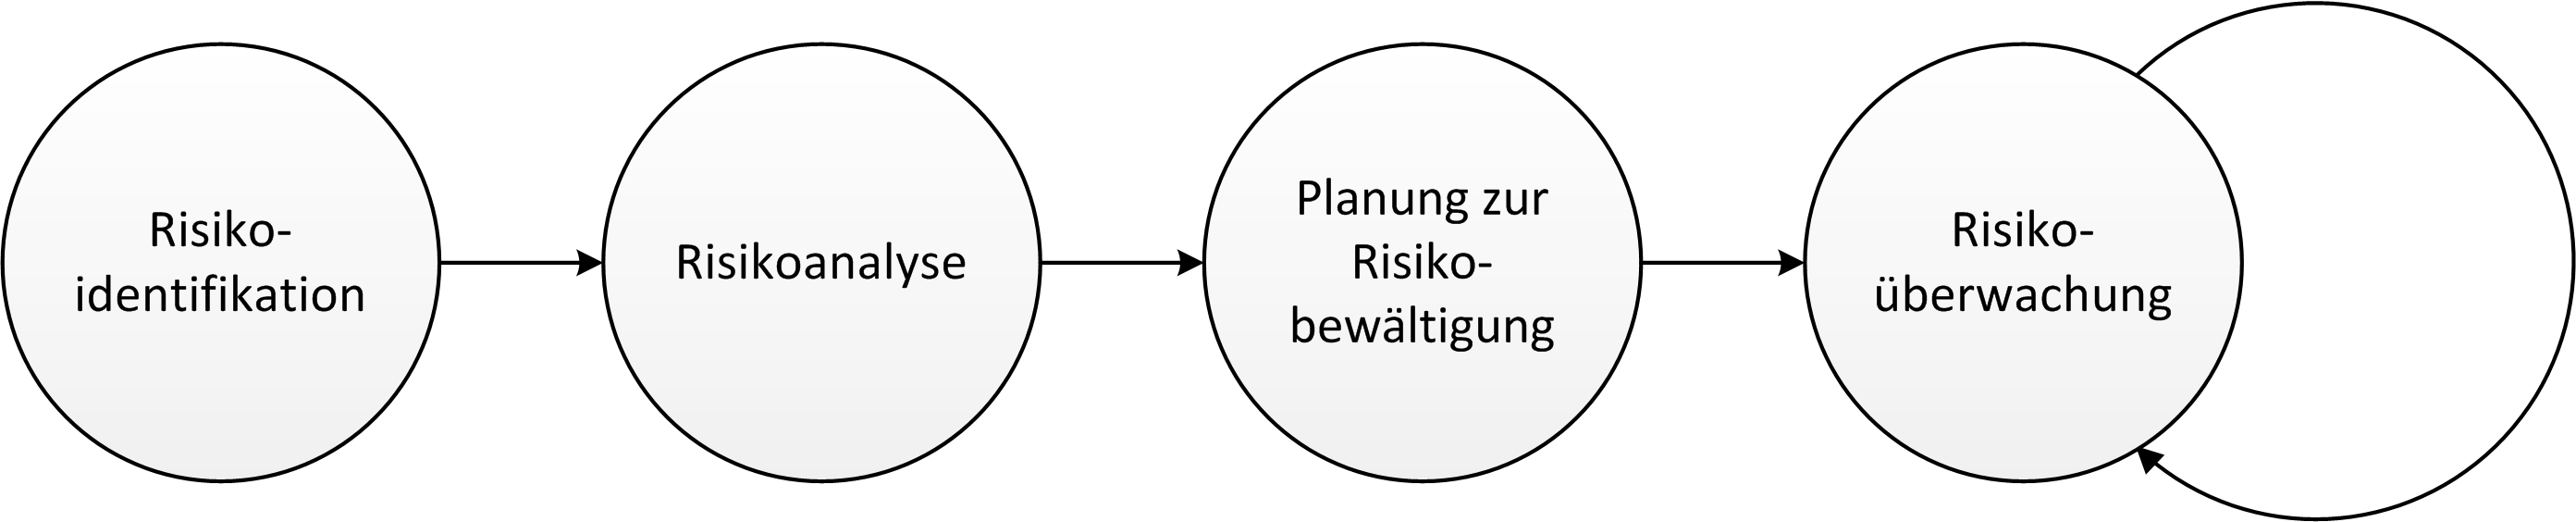
\includegraphics[width=0.8\textwidth]{Illustrationen/2-Methodik/Risikomanagement.png}
	\caption{Risikomanagement Prozess}
	\label{fig:Risikomanagement}
\end{figure}

Im folgenden Abschnitt sind die Prozess kurz erklärt:

\begin{itemize}
	\item \textbf{Risikoidentifikation:} Zu Anfang werden mögliche Risiken identifiziert. Dabei beziehen sich die Risiken im Umfang dieses Projekts auf folgende drei verschiedene Kategorien: soziale Risiken, allgemeine Risiken sowie technische Risiken.
	\item \textbf{Risikoanalyse:} In dieser Phase werden die aufgeschriebenen Risiken kategorisiert. Dabei wird jedes Risiko nach Eintrittswahrscheinlichkeit und Auswirkungen beurteilt. Jedem der beiden Attribute wird ein Zahlenwert, repräsentativ für die Einstufung der Gefahr zugeteilt. Das Produkt der Faktoren für Eintrittswahrscheinlichkeit und Auswirkung stellt dann den Risikograd dar.
	\item \textbf{Planung zur Risikobewältigung:} Für die Risikobewältigung wurden verschiedene Vorgehensweisen definiert. Für Risiken mit geringem Risikograd werden keine Massnahmen definiert. Ab einem mittleren Risikograd sind Massnahmen zur Lösung der potentiellen Probleme zu bestimmen. Bei einem hohen Risikograd sind Präventiv-Massnahmen zu ergreifen, welche die Eintrittswahrscheinlichkeit des entsprechenden Risikos verringern oder gar eliminieren.
	\item \textbf{Risikoüberwachung:} Um ein adäquates Risikomanagement betreiben zu können, müssen die definierten Risiken ständig überwacht werden. Allenfalls sind durch sich ändernde Gegebenheiten neue Risiken zu definieren. In solch einem Fall muss der Risikomanagement Prozess für das betreffende Risiko erneut durchlaufen werden.
\end{itemize}

Das gemäss dieser Vorgehensweise erarbeitet Risikomanagement Dokument ist im Anhang zu finden.